\subsection{Lineaarialgebra (lähteitä)}
Vektoriavaruuden $\mathbb{R}^m$ aliavaruuden $\mathbb{V}$ virittävät keskenään lineaarisesti riippumattomat vektorit $\{\mathbf{a_1,...,a_n}\}$, jota merkitään $\text{span}(\mathbf{a_1,...,a_n})$. Tällöin vektorit $(\mathbf{a_1,...,a_n})$ muodostavat aliavaruuden $\mathbb{V}$ kannan. Vektorit $\{\mathbf{a_1,...,a_n}\}$ ovat keskenään ortogonaalisia, jos ne ovat kohtisuorassa toisiaan vastaan. Ne ovat lisäksi ortonormaaleja, jos ne ovat yksikkövektoreita eli $||\mathbf{a}_i||=1$.

Olkoon matriisi $\mathbf{A}\in \mathbb{R}^{m\times n}$, jonka rivien lukumäärä on $\mathit{m}$ ja sarakkeiden $\mathit{n}$. Merkintä $\mathbf{A}(:,i)$ tarkoittaa matriisin \textbf{A} \textit{i}:ttä saraketta ja vastaavasti $\mathbf{A}(i,:)$ \textit{i}:ttä riviä. Matriisin \textbf{A} virittävät sen lineaarisesti riippumattomat sarakevektorit eli $\text{span}(\mathbf{A}) = \text{span}(\mathbf{A(:,1)},...,A(:,n)) = \text{span}(\mathbf{A}(:,1:n)$. 

Matriisin \textbf{A} aste eli $\text{rank}(\textbf{A})$ kuvaa matriisin lineaarisesti riippumattomien sarake- tai rivivektoreiden lukumäärää. Matriisi \textbf{A} on kääntyvä eli sillä on käänteismatriisi $\mathbf{A}^{-1}$, jos matriisin aste on yhtä kuin sen rivien tai sarakkeiden määrä eli $\text{rank}(\textbf{A})=m=n$.

Singulaariarvohajotelman avulla matriisi voidaan esittää sen ominaisarvojen ja ortonormaalien matriisien avulla

\begin{equation}
    \mathbf{A = UDV^T,}
\end{equation}
jossa matriisin $\mathbf{A}$ ominaisarvot ovat matriisin $\mathbf{D}$ diagonaalilla. Ominaisarvoja $d_i$ on matriisin $\mathbf{D}$ diagonaalilla yhtä paljon, kuin matriisilla $\mathbf{A}$ on lineaarisesti riippumattomia sarakkeita. Toisin sanoen ominaisarvojen joukko on $\{d_1,...,d_r\}$, jossa $r = \text{rank}(\mathbf{A})$. Loput luvut matriisin \textbf{D} diagonaalilla ovat nollia. Singulaariarvohajotelma voidaan näin esittää matriisitulon avulla 

\begin{equation}
    \mathbf{A} = \mathbf{U}(:,1:r)\mathbf{D}(1:r,1:r)\mathbf{V}(:,1:r)^T
    \label{eq:2}
\end{equation}


Pseudokäänteismatriisi $\mathbf{A^{\dagger}}$ on yleistys matriisin käänteismatriisille. Tämä joudutaan muodostamaan silloin, kun matriisi $\mathbf{A}$ ei ole kääntyvä. Pseudokäänteismatriisi saadaan muodostettua singulaariarvohajotelman avulla

\begin{equation}
    \mathbf{A^{\dagger} = VD^{\dagger}U^T}
\end{equation}

Projektio aliavaruuteen $\text{span}(\mathbf{A})$ saadaan kaavalla

\begin{equation}
    \mathbf{\Pi}_{\text{span}(\mathbf{A})}= \mathbf{AA}^{\dagger}
\end{equation}

ja tämän ortogonaaliseen aliavaruuteen saadaan

\begin{equation}
    \mathbf{\Pi}_{\text{span}(\mathbf{A}^{\bot})}=\mathbf{I}-\mathbf{AA}^{\dagger}
\end{equation}

Ortogonaalisen matriisin sarakkeet ja rivit ovat ortonormaaleja (lähde?). Täten ortogonaalisen matriisin \textbf{U} sarakkeet $\mathbf{U}(:,1),...,\mathbf{U}(:,r)$ muodostavat ortonormaalin kannan matriisille \textbf{A} eli $\text{span}(\mathbf{A}) = \mathbf{U}(:,1:r)$. Projektio aliavaruuteen $\text{span}(\mathbf{A})$ voidaan nyt muodostaa singulaariarvohajotelman avulla

\begin{equation}
    \mathbf{\Pi}_{\text{span}(A)} = \mathbf{U}(:,1:r)\mathbf{U}(:,1:r)^T,
    \label{eq:6}
\end{equation}
jossa $\mathbf{U}(:,1:r)^T = \mathbf{U}(:,1:r)^{\dagger}$.

\begin{figure}[h]
    \centering
    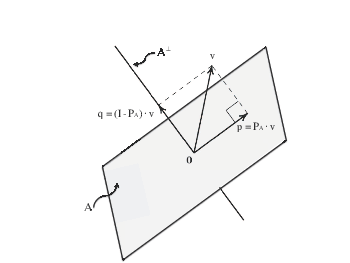
\includegraphics[width=.7\textwidth]{ortoprojektio.png}.
    \caption{Ortoprojektio}
\end{figure}